\documentclass{article}

\usepackage{amsmath,amssymb}
\usepackage{multicol}
\usepackage{systeme}
\usepackage{url}
%\usepackage{siunitx}

% for drawing graphs
\usepackage{tikz}
\tikzset{every picture/.style={thick}}
\tikzset{every node/.style={draw, circle, inner sep = 2pt}}
\usetikzlibrary{arrows}

% for margins
\usepackage[margin=1in]{geometry}

% for font
\usepackage{euler}
\usepackage[OT1]{eulervm}
\renewcommand{\rmdefault}{pplx}

\setlength{\parindent}{0pt}  %no indenting

% MACROS
\newcommand{\trans}{^\top}
\newcommand{\adj}{^{\rm adj}}
\newcommand{\cof}{^{\rm cof}}
\newcommand{\inp}[2]{\left\langle#1,#2\right\rangle}
\newcommand{\dunion}{\mathbin{\dot\cup}}
\newcommand{\bzero}{\mathbf{0}}
\newcommand{\bone}{\mathbf{1}}
\newcommand{\ba}{\mathbf{a}}
\newcommand{\bb}{\mathbf{b}}
\newcommand{\bd}{\mathbf{d}}
\newcommand{\be}{\mathbf{e}}
\newcommand{\bp}{\mathbf{p}}
\newcommand{\bq}{\mathbf{q}}
\newcommand{\bx}{\mathbf{x}}
\newcommand{\by}{\mathbf{y}}
\newcommand{\bz}{\mathbf{z}}
\newcommand{\bu}{\mathbf{u}}
\newcommand{\bv}{\mathbf{v}}
\newcommand{\bw}{\mathbf{w}}
\newcommand{\tr}{\operatorname{tr}}
\newcommand{\nul}{\operatorname{null}}
\newcommand{\rank}{\operatorname{rank}}
%\newcommand{\ker}{\operatorname{ker}}
\newcommand{\range}{\operatorname{range}}
\newcommand{\Col}{\operatorname{Col}}
\newcommand{\Row}{\operatorname{Row}}
\newcommand{\spec}{\operatorname{spec}}
\newcommand{\vspan}{\operatorname{span}}
% \newenvironment{sol}{\medskip\noindent {\bf Solution.}}{\newpage}
\newcommand{\mystrut}{\rule[-.5\baselineskip]{0pt}{2\baselineskip}}
% \newcommand{\mul}{\operatorname{mul}}
\newcommand{\even}{\operatorname{even}}
\newcommand{\sgn}{\operatorname{sgn}}
\newcommand{\iner}{\operatorname{iner}}
\newcommand{\rL}{\mathring{L}}
\newcommand{\diag}{\operatorname{diag}}

\makeatletter
%%%The definition of \binom is \genfrac ()\z@ {}
%%%To adjust the spaces between parantheses, change the augment of \kern
\newcommand{\multiset}[2]{\ensuremath{\left(\kern-.3em\left(\genfrac{}{}{\z@}{}{#1}{#2}\right)\kern-.3em\right)}}
\newcommand{\qanalog}[2]{\genfrac []\z@ {}{#1}{#2}_q}
\makeatother

% for title
\title{2021F Math585 Midterm1}
\date{\vspace{-1cm}}
\begin{document}
\maketitle
\large

\textbf{4 questions}, \textbf{20 total points}

\textbf{Note:}  Use other papers to answer the problems.  Remember to write down your \textbf{name} and your \textbf{student ID \#}.

\begin{enumerate}
\setlength\itemsep{2em}

\item{} [5pt] The weighted digraph below represents a matrix, where each edge has weight $1$, while the numbers $x_1, \ldots, x_6$ nearby the nodes represent a vector.  Find the product of the matrix and the vector, and then draw the product.

\begin{center}
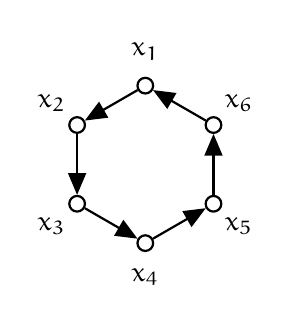
\begin{tikzpicture}
\foreach \i in {1,...,6} {
    \pgfmathsetmacro{\ang}{90 + 60*(\i - 1)}
    \node[label={\ang:$x_{\i}$}] (\i) at (\ang:1) {}; 
}
\draw[-triangle 45] (1) -- (2);
\draw[-triangle 45] (2) -- (3);
\draw[-triangle 45] (3) -- (4);
\draw[-triangle 45] (4) -- (5);
\draw[-triangle 45] (5) -- (6);
\draw[-triangle 45] (6) -- (1);
\end{tikzpicture}
\end{center}

\item{} [5pt] Let  
\[
    A = \begin{bmatrix}
    1 & 1 & 0 & 0 & 0 \\
    0 & 1 & 1 & 0 & 0 \\
    0 & 0 & 1 & 1 & 0 \\
    0 & 0 & 0 & 1 & 1 \\
    1 & 0 & 0 & 0 & 1
    \end{bmatrix}.
\]
Find the $1,1$-entry of $A^5$ and the $1,1$-entry of $A^{100}$.  \label{item:A}

\item{} [5pt] Let $A$ be the matrix as in Problem~\ref{item:A}.  Find $\det(A)$.  

\item{} [5pt] Let $A$ be the matrix as in Problem~\ref{item:A}.  Find the characteristic polynomial $\det(A - xI)$.  

% \vfill

% \textbf{One more problem on the back.}

% \newpage

\end{enumerate}



\end{document}



  
